\section{Data}
% are all the acronyms too much?
% TODO time and diurnal (?)
% TODO figure for regions
% TODO rainfall data
\begin{table}
  \centering
  \resizebox{0.85\linewidth}{!}{%
  \begin{tabular}{ l c c c }
    \toprule
    Channel & $\lambda_{\mathrm{cen}}$ ($\mu$m) & $\lambda_{\mathrm{min}}$ ($\mu$m) & $\lambda_{\mathrm{max}}$ ($\mu$m) \\
    \midrule
    VIS0.6  & 0.64                    & 0.56                    & 0.71                    \\
    VIS0.8  & 0.81                    & 0.74                    & 0.88                    \\
    NIR1.6  & 1.64                    & 1.50                    & 1.78                    \\
    \bottomrule
  \end{tabular}}
  \caption{Spectral characteristics of the three SEVIRI channels used
    in our work. Shown are the central, minimum and maximum
    wavelengths for the three spectral bands that we use.}
  \label{tab:seviri}
\end{table}

This work mainly comprises of analysing data products that we have
produced using raw data from the European Organisation for the
Exploitation of Meteorological Satellites
(EUMETSAT) \footnote{\url{https://www.eumetsat.int}}. In particular,
we have utilised the Meteosat Second Generation (MSG) series of
meterological satellites, which provide continous observations of the
full disk of the Earth via the Spinning Enhanced Visible and Infrared
Imager (SEVIRI) \citep{schmetz2002}. MSG is in an equatorial
geostationary orbit fixed at $0^{\circ}$ longitude and makes observations
every 15 minutes in 12 spectral bands, returning images $3712 \times 3712$
pixels in size. Not all of the 12 available bands are useful for our
investigation -- the spectral responses of the three bands that we use
are detailed in Table \ref{tab:seviri}. For consistency, we use data
collected at 12:00 each day, since this is the time when land is the
most illuminated.

\begin{table}
  \centering
  \resizebox{\linewidth}{!}{%
  \begin{tabular}{ l c c c c }
    \toprule
    \multirow{2}{*}{Region} &
    \multicolumn{2}{c}{Latitude (deg)} &
    \multicolumn{2}{c}{Longitude (deg)} \\
                 & {Top} & {Bottom} & {Left} & {Right}    \\
    \midrule
    South Africa & $-21.501$ & $-35.659$ & 14.728 & 33.193 \\
    East Africa  & 10.085    & 1.615     & 34.518 & 46.071 \\
    \bottomrule
  \end{tabular}}
  \caption{The coordinates that define our regions of interest. Top
    (Left) and Bottom (Right) correspond to the most northern
    (eastern) and southern (western) latitudes (longitudes) of the
    boxes defining the regions, respectively. All values in decimal
    degrees.}
  \label{tab:regions}
\end{table}

The full Earth image as collected by EUMETSAT is not terribly useful
in its original form for two reasons:
\begin{itemize}
  \item{it is quite a large
    image and so memory considerations alone make processing the whole
    image a difficult task;}
  \item{any effect that \elnino\ has on African climate is likely to be
    quite localised and, at the very least, we expect the trends to be
    reversed on either side of the equator.}
\end{itemize}
To address these challenges, we have defined two regions of interest
(selected after \cite{anyamba1996, anyamba2002}) in southern and
eastern Africa. The exact boundaries of these regions are listed in
Table \ref{tab:regions}. In addition, since we will be investigating
vegetation coverage, we restrict our study to continental areas using
the land mask provided by EUMETSAT.
\begin{figure}
  \centering
  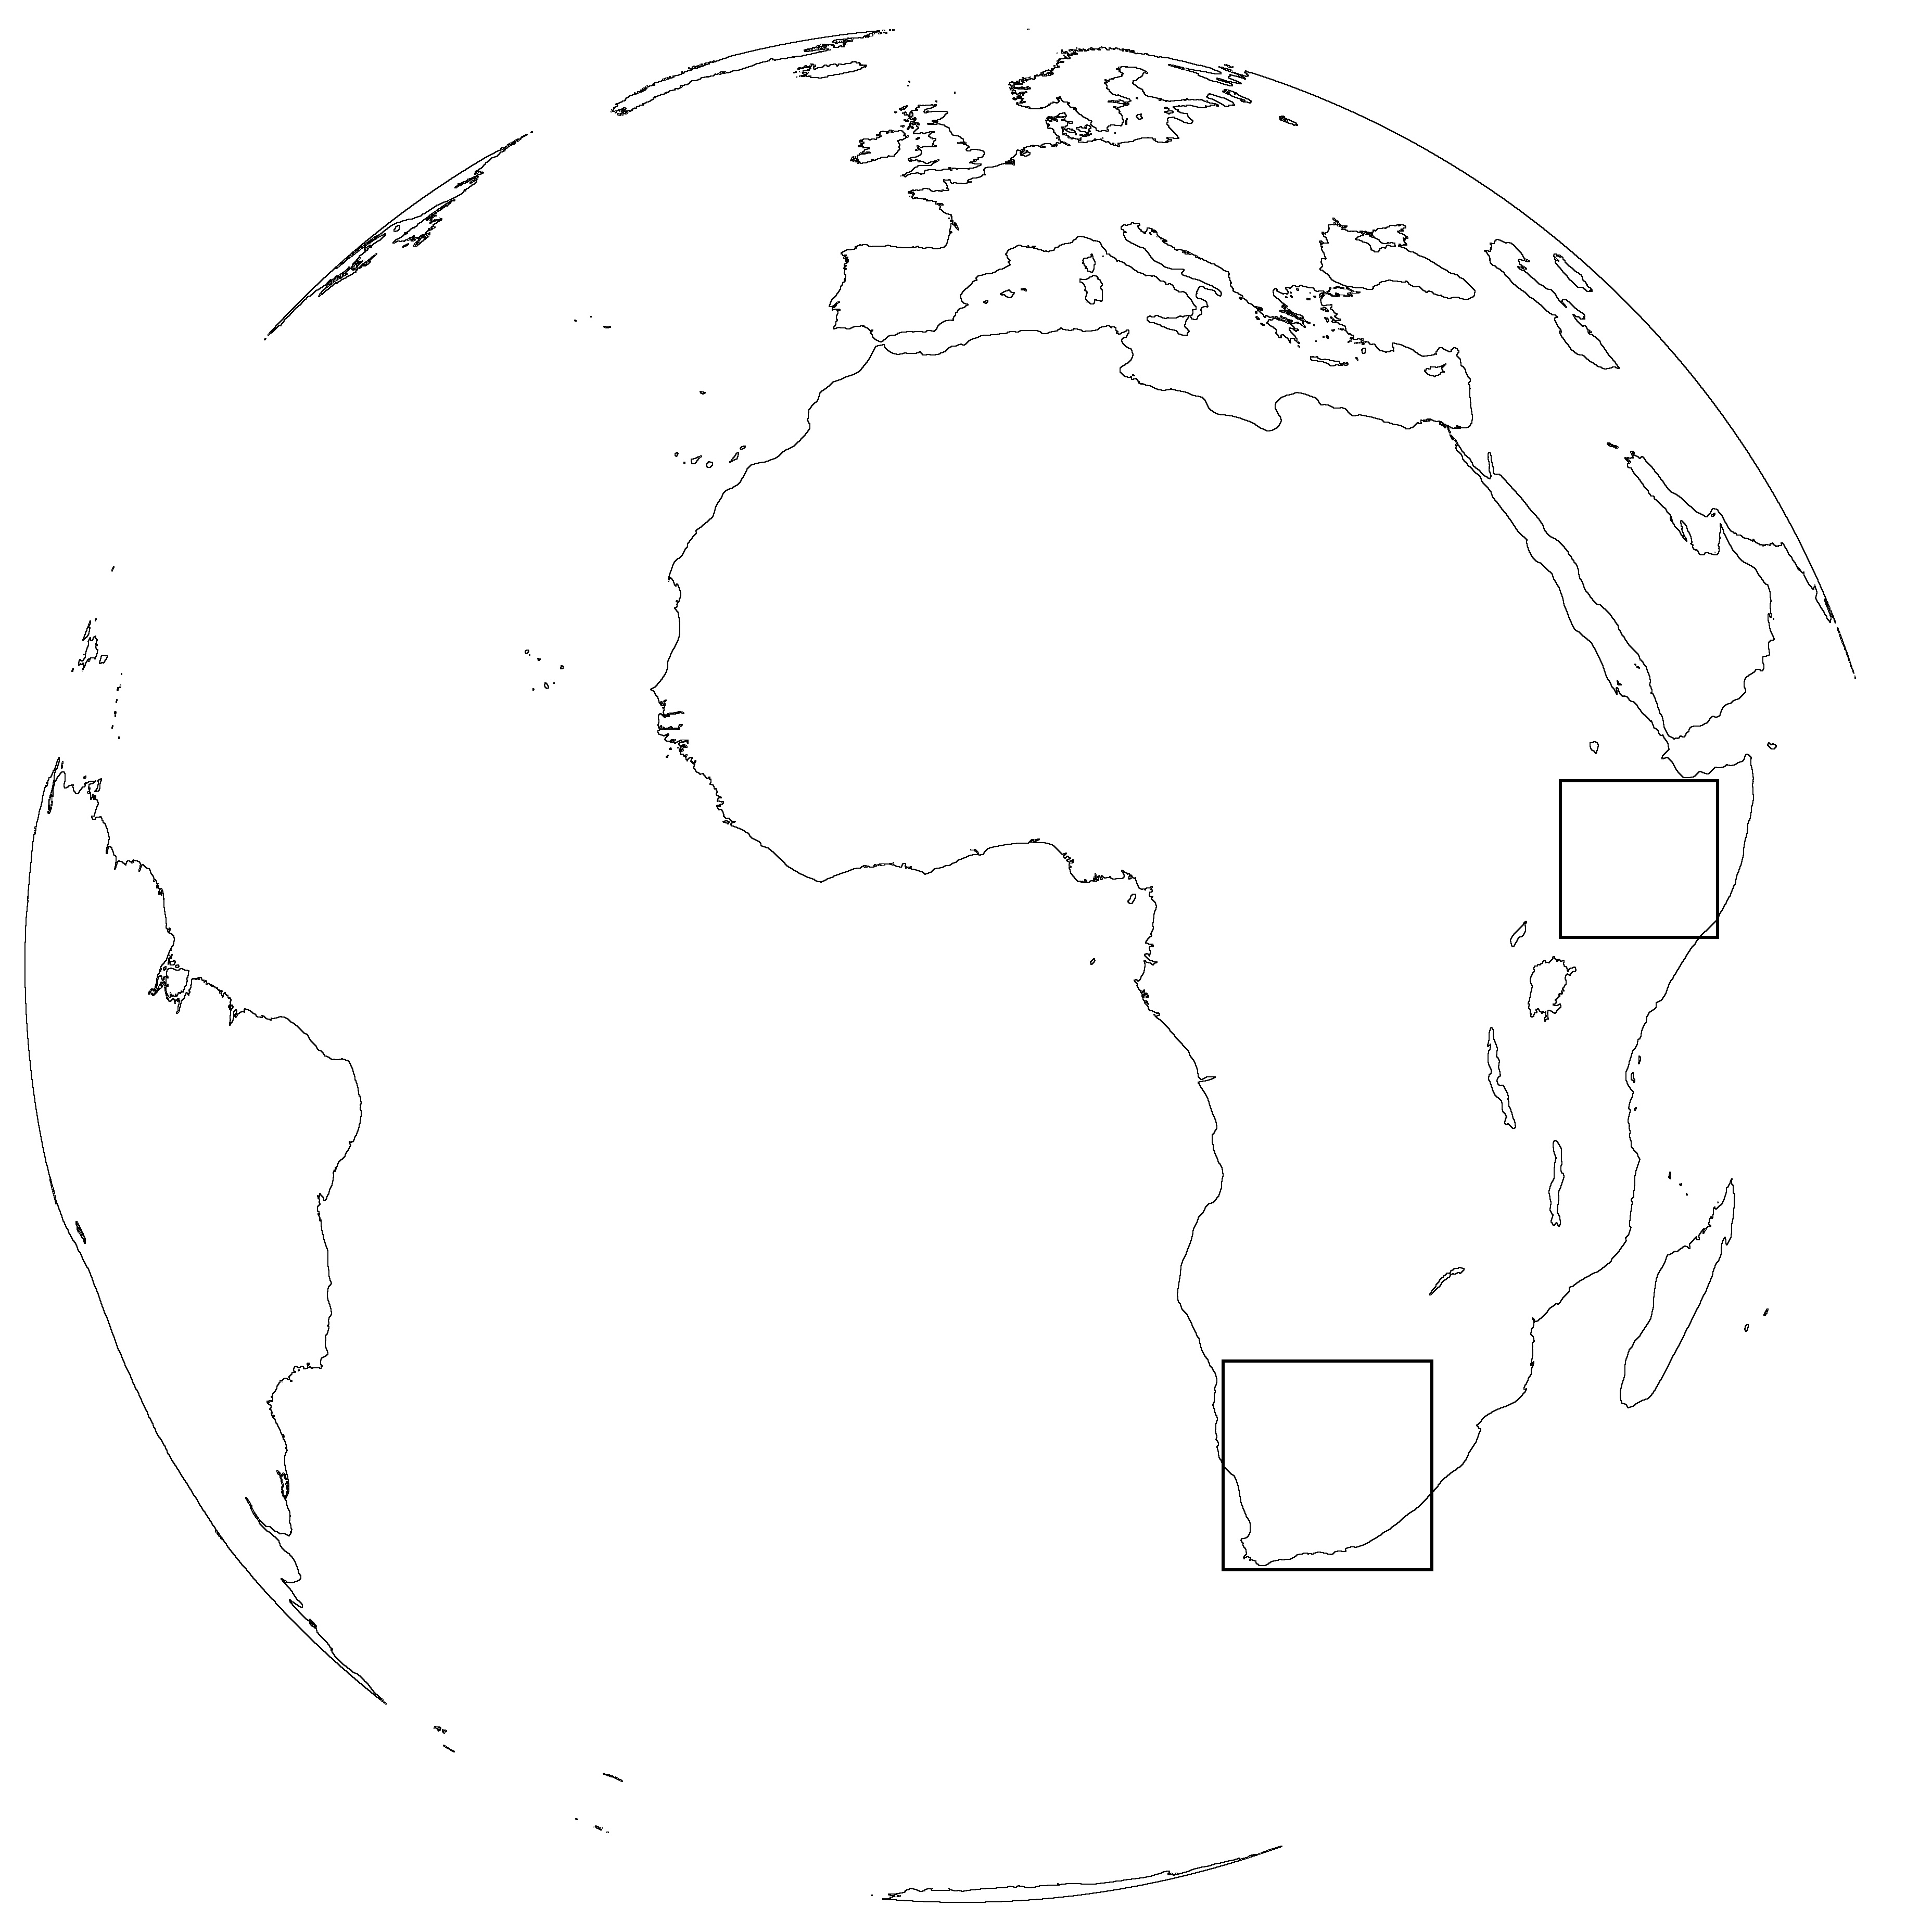
\includegraphics[width=0.9\linewidth]{figures/regions_figure}
  \caption{The EUMETSAT land mask image after using Sobel kernels to
    detect edges. The two black squares indicate the regions defined
    in Table \ref{tab:regions}.}
  \label{fig:regions}
\end{figure}
We also make use of data provided from other sources. For sea surface
temperature (SST) anomalies, we use the time series anomalies provided
by the National Oceanic and Atmospheric Administration
(NOAA) \footnote{\url{https://stateoftheocean.osmc.noaa.gov/}}. NOAA
provide SST anomalies for the Indian Ocean (IO) in the South Western
(SWIO) and Western Tropical (WTIO) regions, as well as Ni{\~n}o 3.4
SST anomalies. SWIO and WTIO anomalies are smoothed by taking three
month means, and the SWIO anomalies are compared to the data for South
Africa while the WTIO anomalies are compared to East Africa. We use
the anomalies in this way because each IO region is in close proximity
to its corresponding continental region, so it is reasonable to expect
that the anomalies may directly impact the continental climate. The
Ni{\~n}o 3.4 anomalies can be processed into the Oceanic Ni{\~n}o
Index (ONI) by smoothing with three monthly means, much in the same
way as the IO anomalies. \elnino\ events are then said to occur when
the ONI surpasses $0.5^{\circ}$C for at least five consecutive three
monthly periods. \nina\
conditions are present when the ONI falls
below $-0.5^{\circ}$C for the same time conditions.

The final tool in our complement of climate measures is rainfall
data. This is provided by the World
Bank \footnote{\url{http://www.worldbank.org/}} and we use it to
examine the extent to which cloud coverage is useful as a proxy
measure for rainfall.

\subsection{Calibration}
\label{sec:data:calib}

The images we are processing are provided by \emph{EUMETSAT} as
\emph{PNG} data, where each pixel may take a value in the range
$\left[0, 255\right]$ as is common for PNG data. Ideally, the data
would be provided in the units of \emph{radiance}
(Wm$^{-2}$sr$^{-1}$(cm$^{-1}$)$^{-1}$) being a measure of the amount
of incident light received by the sensor. Howevever, the pixel values
are \emph{not} expressed in physical values: they are instead the
pixel \emph{count}, representing how often a particular element of the
satellite's sensor (charge-coupled device, or CCD) was
activated. While this value is useful and intuitive for diagrammatic
uses, the sensors response to incident light is not constant over the
various spectral bands being observed. As is described in Section
\ref{TODO}, our \emph{NDVI} analysis will use data from two different
bands (namely \emph{VIS8} and \emph{VIS6}) and so we have to be
careful when comparing the two.

The \emph{MSG} satellites perform callibration using an on-board
\emph{black-body} source. For each of the channels, two values are
calculated for every image:
\begin{enumerate}
\item \emph{Cal\_Offset}: the radiance value for a pixel count of
  zero; and
\item \emph{Cal\_Slope}: how radiance varies with pixel count.
\end{enumerate}
This calibration data is provided by EUMETSAT in separate header files
(\emph{LRIT} and \emph{HRIT}). The obscure software \texttt{xrit2pic}
was used to read in these header files so that we may pull out the
above calibration values.

On the constancy of \emph{Cal\_Offset} and \emph{Cal\_Slope} over time
\cite{muller2007msg} has the note (emphasis added) ``The data is \dots
kept constant for an image but is likely to be updated from one image
to the next (\textbf{although it is expected to vary only slowly}).''
Indeed, upon inspection the calibration values were not observed to
change over a period of time. While this was not tested over the
entirety of the data, we decided in the interest of time that the
above quote and cursory test were justification enough that we could,
at this time, take as constant the calibration values. Thus we chose
for the calibration values those shown in Table \ref{tab:calibration}.
% TODO Perhaps add a note for future work that would include the true
% calibration values / show that they do not vary significantly enough
% to warrant inclusion.

\begin{table}
  \centering
  \resizebox{0.6\linewidth}{!}{%
  \begin{tabular}{ r c c }
    \toprule
    Channel & \emph{Cal\_Offset} & \emph{Cal\_Slope} \\
    \midrule
    VIS0.6 & 1 & 1 \\
    VIS0.8 & 1 & 1 \\
    NIR    & 1 & 1 \\
    \bottomrule
  \end{tabular}}
  \caption{Calibration values for each band. It is assumed that these
    values vary only slowly, and so we have decided to use a single
    set of values.}
  \label{tab:calibration}
\end{table}

Calibration of pixel value to physical radiance value is then
performed with the calculation
\begin{equation}
    \textrm{R}_{i,\textrm{channel}} = \textrm{CO}_\textrm{channel} +
    \textrm{CS}_\textrm{channel} \times
    \textrm{PC}_i \label{eqn:calibration}
\end{equation}
where R$_{i,\textrm{channel}}$ is the calibrated radiance value for
pixel $i$ in the channel, CO$_\textrm{channel}$ and
CS$_\textrm{channel}$ are the calibration offset and slope
respectively, and PC$_i$ is the pixel count for pixel $i$.

\subsubsection{Radiance and Reflectance}

It is not \emph{strictly} true that NDVI is calculated with
radiance. In many publications NDVI is calculated using
\emph{reflectance}. Radiance measures the amount of light incident on
the sensor which is necessarily subject to multiple sources of
interference such as the Earth's atmosphere for example. It is the
case then that we are not measuring an intrinsic property of the light
source -- it's reflectance -- instead we are measuring a property of the
sensor. Reflectance is the ratio of light radiated by the object to
the light incident upon the object.

The reflectance $r_{\lambda_i}$ for band $\lambda_i$ can be calculated from
radiance $R_{\lambda_i}$ using the \emph{Bidirectional Reflectance Factor}
formula \citep{msgbdrf2012}
\begin{align}
  r_{\lambda_i} &= \frac{\pi \cdot R_{\lambda_i} \cdot d^2\left(t\right)} {I_{\lambda_i} \cdot
    \cos\left(\theta\left(t, x\right)\right)}
\end{align}
where $d^2\left(t\right)$ is the Earth-Sun distance (AU) at time $t$,
$I_{\lambda_i}$ is the solar irradiance (a constant determined by
calibration), and $\cos\left(\theta\left(t, x\right)\right)$ is the solar
zenith angle at time $t$ and position $x$.

We have elected to forgo this conversion, reasoning that
$d^2\left(t\right)$ is \emph{roughly} constant (fractional change
between aphelion and perihelion is ${\sim}3\%$), and that the extent of
Africa is approximately $30^{\circ}$N--$30^{\circ}$S and
$15^{\circ}$W--$45^{\circ}$E. The contribution of these factors is then small
enough that we may furtively ignore them. Less furtively
\cite{ray1994} states ``For most of the vegetation indices \dots
radiance, reflectance, and apparent reflectance can be used
interchangibly.''

\subsection{Bands used in NDVI}

While the particular choice of central wavelength differs between
publications, the bands used in NDVI calculations are often described
in literature is \emph{near infrared} (NIR) and \emph{red} (R)
bands. We note here that this may lead to confusion. For example, we
have three visual bands available for our investigation shown in Table
\ref{tab:seviri}. Na{\"i}vely we may then expect that NDVI
calculations are to be performed with the NIR band corresponding to a
central wavelength of $1.64\mu$m (NIR in Table \ref{tab:seviri}), and R
corresponding to a central wavelength of $0.81\mu$m (VIS0.8 in Table
\ref{tab:seviri}). However, \cite{msgndvi2015} instead adopts for NIR
a value of $0.81\mu$m (VIS0.8 in Table \ref{tab:seviri}), and for R a
value of $0.64\mu$m (VIS0.6 in Table \ref{tab:seviri}).

So it should be kept in mind that wherever in the following NDVI
analysis we refer to ``NIR'' we are infact using the data for
``VIS0.8''; and likewise ``R'' refers to the data for ``VIS0.6''.

%% Local Variables:
%% fill-column: 80
%% TeX-master: "report"
%% End:
